
\chapter{Heatmaps}
\label{cha:heatmaps}

I dette afsnit fremviser vi alle heatmaps der blev gemt under
testen. S�fremt der er et hvidt felt skyldes det at barnet ikke
spillede den p�g�ldende udgave.

\section{\ima}

\begin{figure}[h]
  \centering
  \subfloat[Med KI]{\label{fig:ima1Dai}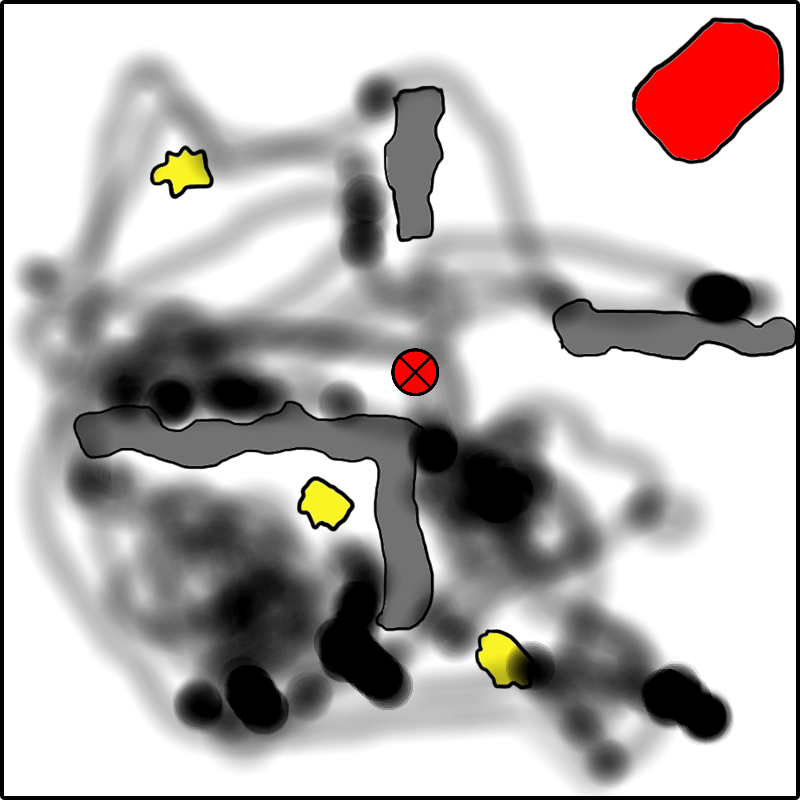
\includegraphics[width=0.4\textwidth]{contents/testing/heatmaps/imachination/1Dai.png}}               \qquad
  \subfloat[Uden KI]{\label{fig:ima1Dnoai}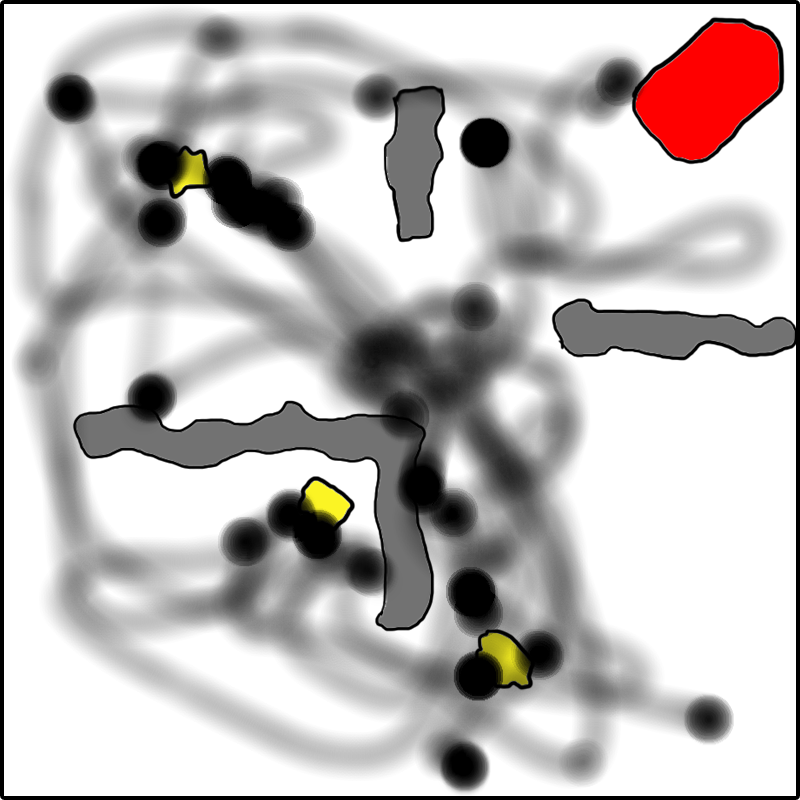
\includegraphics[width=0.4\textwidth]{contents/testing/heatmaps/imachination/1Dnoai.png}}
  \caption{1D \ima spillede uden KI f�rst}
  \label{fig:1Dima}
\end{figure}

\begin{figure}[h]
  \centering
  \subfloat[Med KI]{\label{fig:ima2Pai}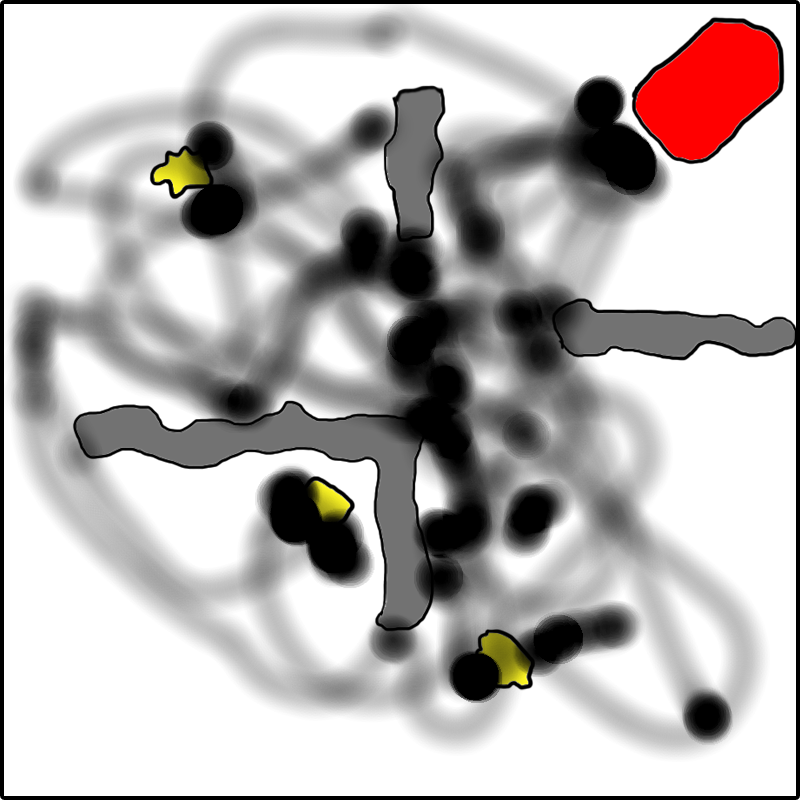
\includegraphics[width=0.4\textwidth]{contents/testing/heatmaps/imachination/2Pai.png}}               \qquad
  \subfloat[Uden KI]{\label{fig:ima2Pnoai}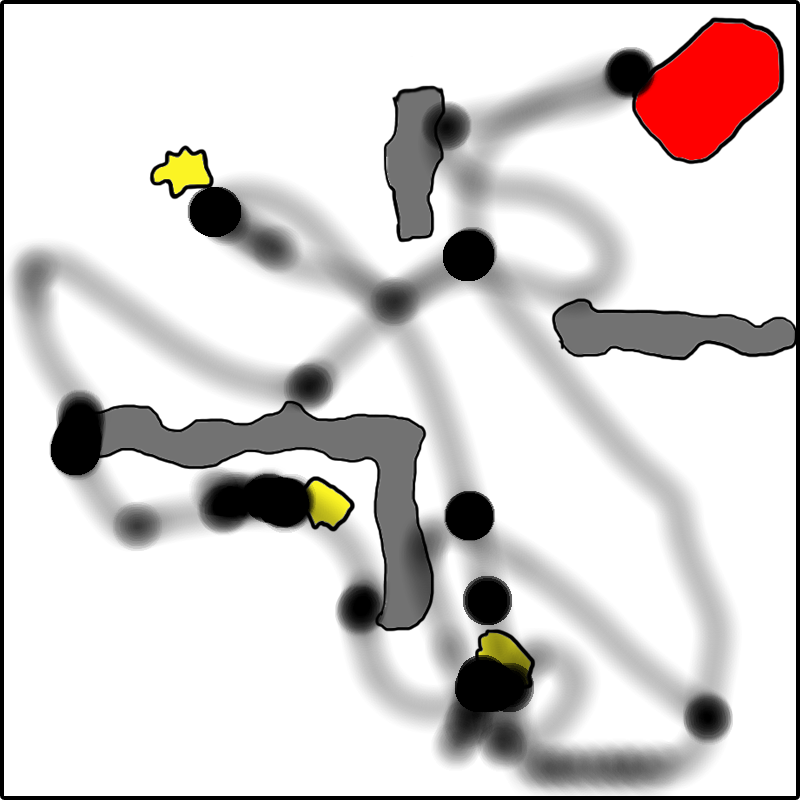
\includegraphics[width=0.4\textwidth]{contents/testing/heatmaps/imachination/2Pnoai.png}}
  \caption{2P spillede med KI f�rst}
  \label{fig:2Pima}
\end{figure}

\begin{figure}[h]
  \centering
  \subfloat[Med KI]{\label{fig:ima3Dai}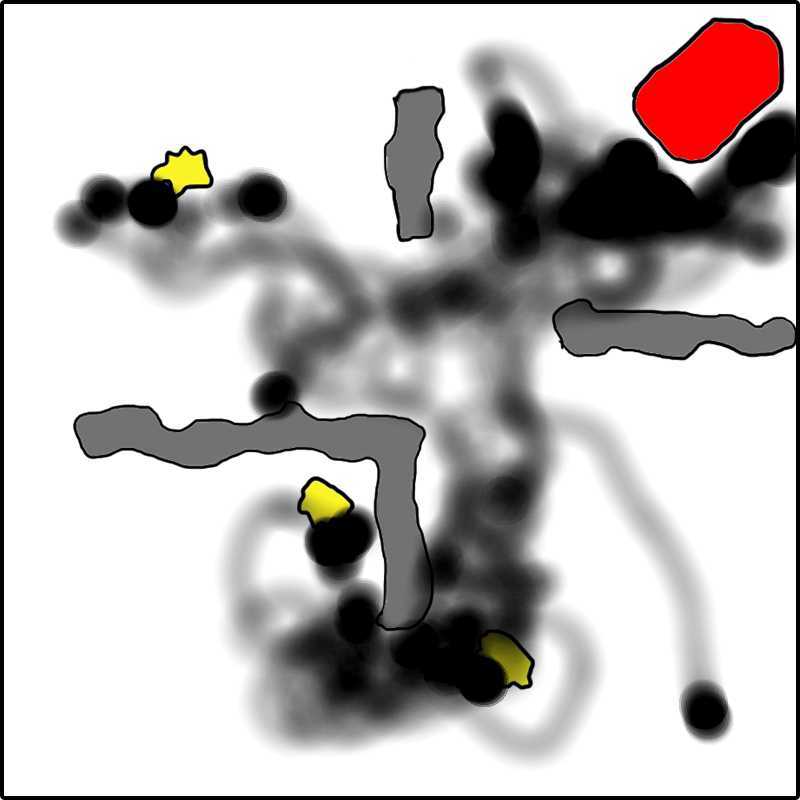
\includegraphics[width=0.4\textwidth]{contents/testing/heatmaps/imachination/3Dai.png}}               \qquad
  \subfloat[Uden KI]{\label{fig:ima3Dnoai}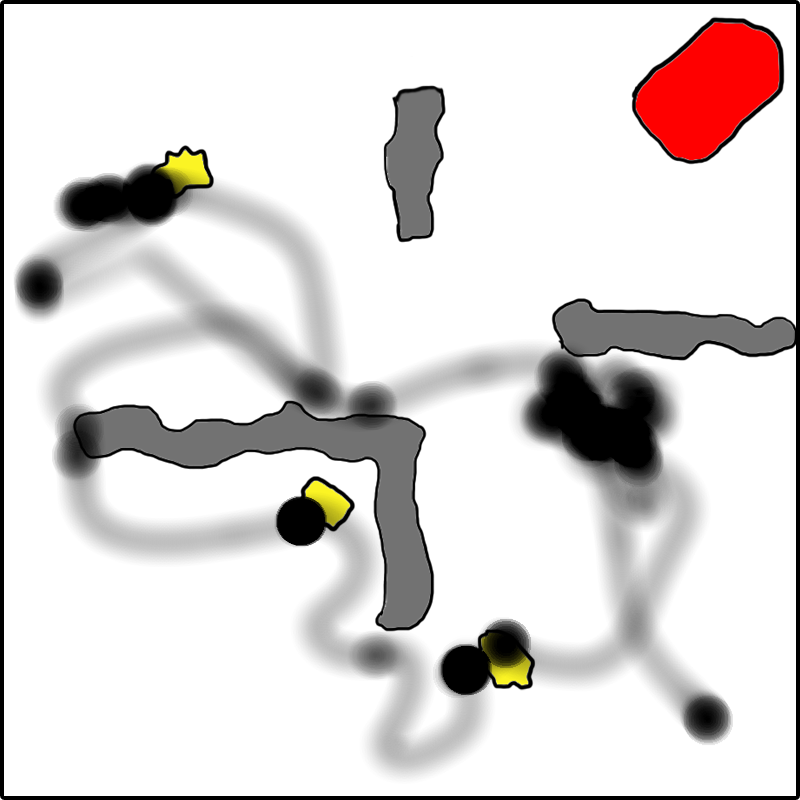
\includegraphics[width=0.4\textwidth]{contents/testing/heatmaps/imachination/3Dnoai.png}}
  \caption{3D spillede med KI f�rst}
  \label{fig:3Dima}
\end{figure}

\begin{figure}[h]
  \centering
  \subfloat[Med KI]{\label{fig:ima4Pai}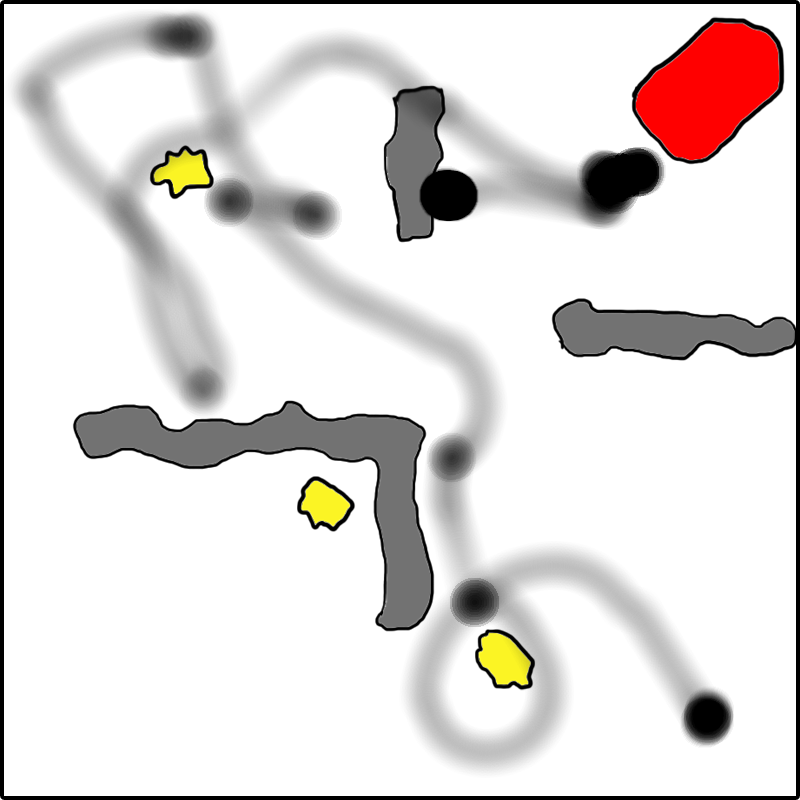
\includegraphics[width=0.4\textwidth]{contents/testing/heatmaps/imachination/4Pai.png}}               \qquad
  \subfloat[Uden KI]{\label{fig:4Pnoai}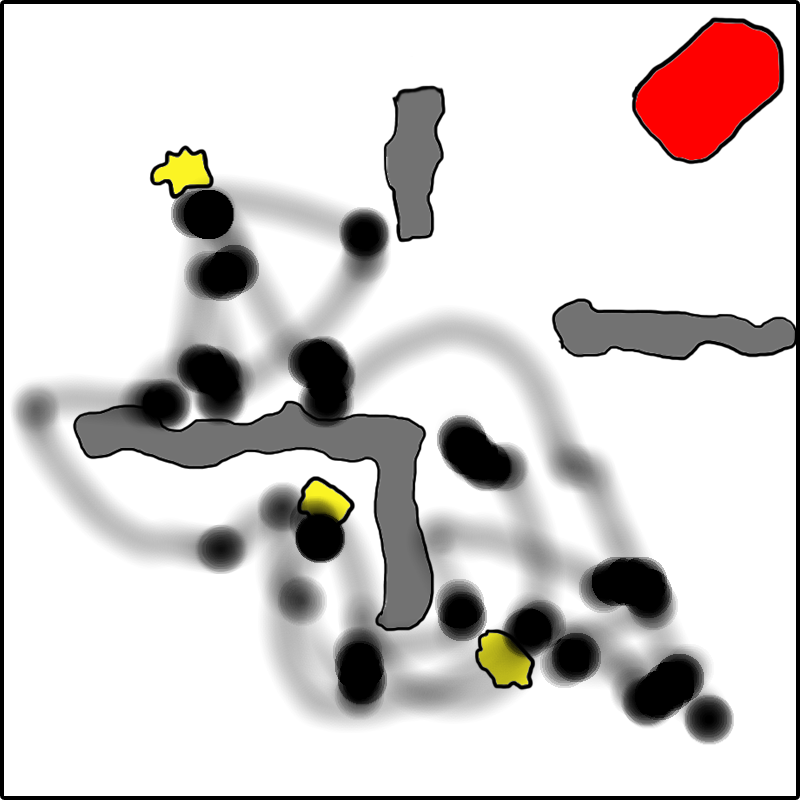
\includegraphics[width=0.4\textwidth]{contents/testing/heatmaps/imachination/4Pnoai.png}}
  \caption{3D spillede med KI f�rst}
  \label{fig:4Pima}
\end{figure}

\begin{figure}[h]
  \centering
  \subfloat[Med KI]{\label{fig:ima5Dai}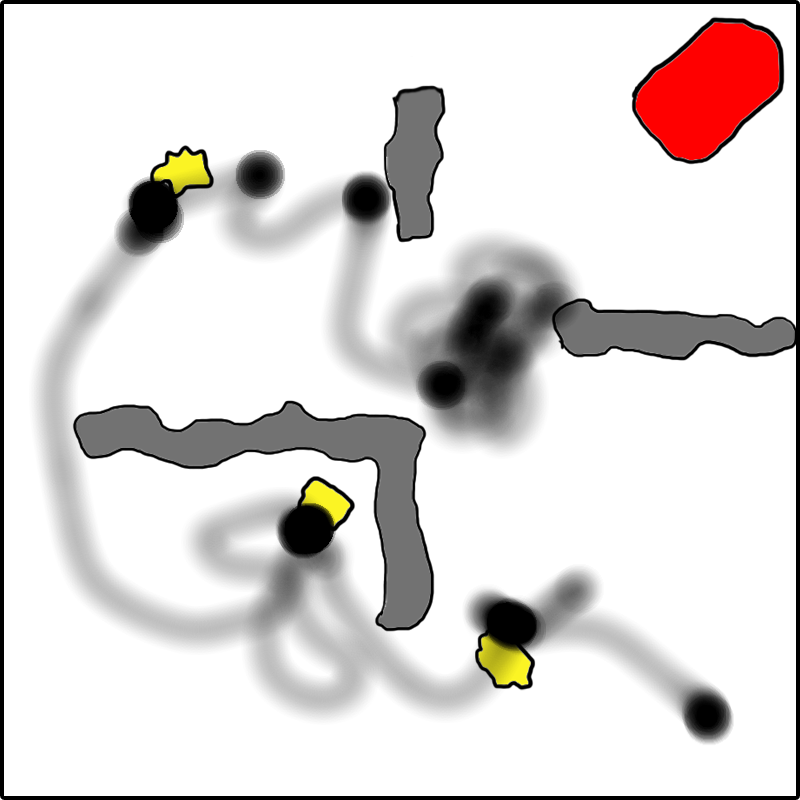
\includegraphics[width=0.4\textwidth]{contents/testing/heatmaps/imachination/5Dai.png}}               \qquad
  \subfloat[Uden KI]{\label{fig:ima5Dnoai}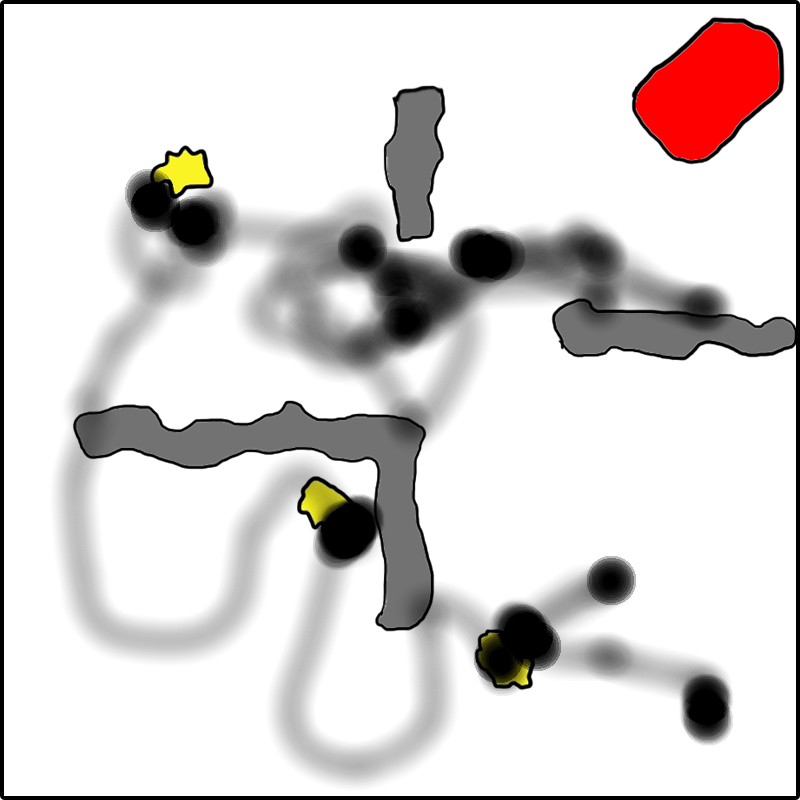
\includegraphics[width=0.4\textwidth]{contents/testing/heatmaps/imachination/5Dnoai.png}}
  \caption{5D spillede uden KI f�rst}
  \label{fig:5Dima}
\end{figure}

\begin{figure}[h]
  \centering
  \subfloat[Med KI]{\label{fig:ima6Dai}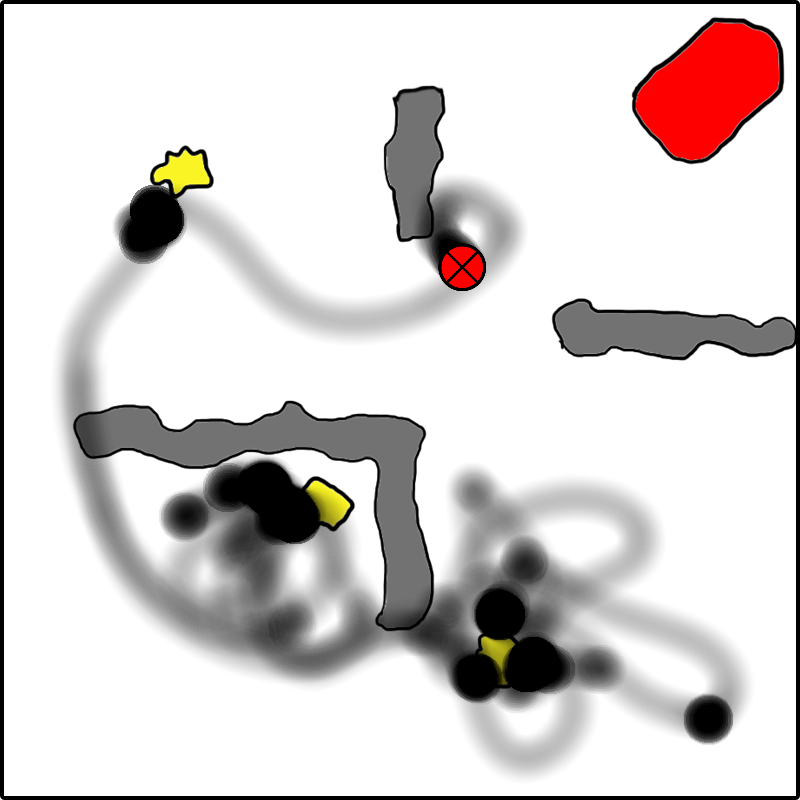
\includegraphics[width=0.4\textwidth]{contents/testing/heatmaps/imachination/6Dai.png}}               \qquad
  \subfloat[Uden KI]{\label{fig:ima6Dnoai}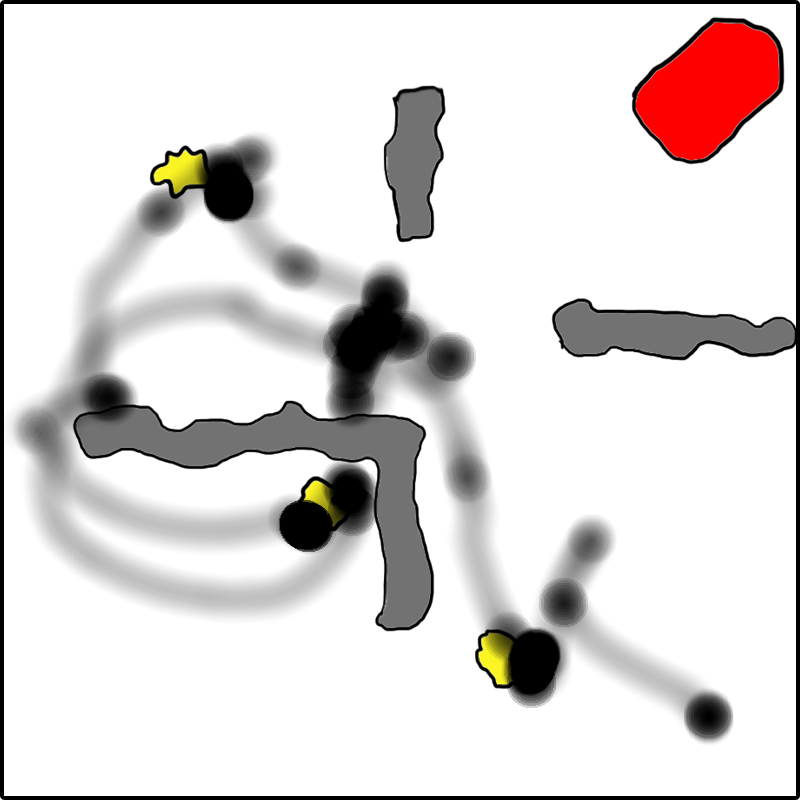
\includegraphics[width=0.4\textwidth]{contents/testing/heatmaps/imachination/6Dnoai.png}}
  \caption{6D spillede uden KI f�rst}
  \label{fig:6Dima}
\end{figure}

\begin{figure}[h]
  \centering
  \subfloat[Med KI]{\label{fig:ima7Dai}
\includegraphics[width=0.4\textwidth]{contents/testing/heatmaps/imachination/7Dai.png}}               \qquad
  \subfloat[Uden KI]{\label{fig:ima7Dnoai}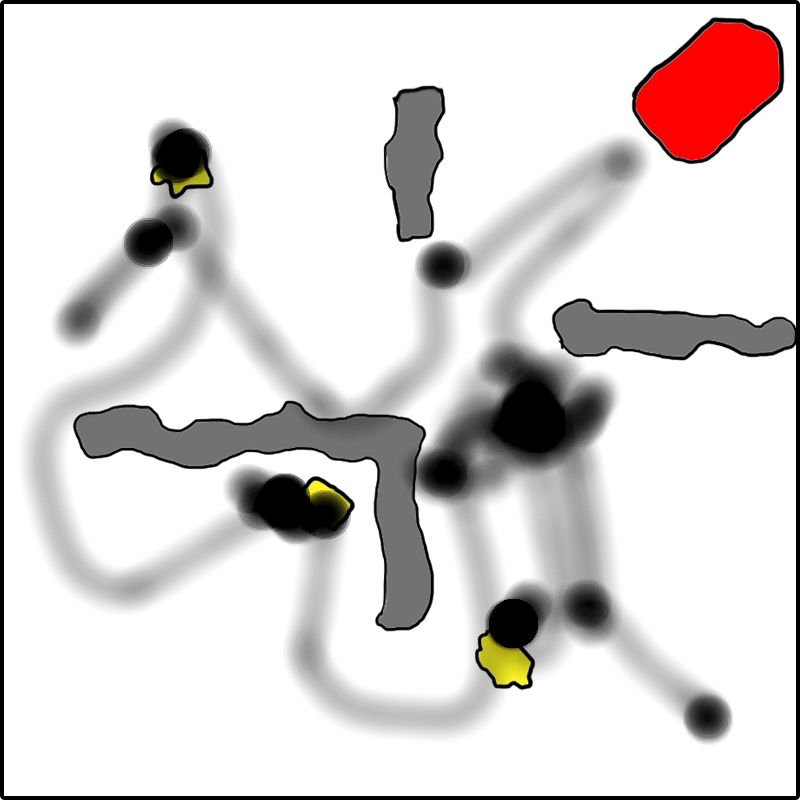
\includegraphics[width=0.4\textwidth]{contents/testing/heatmaps/imachination/7Dnoai.png}}
  \caption{7D spillede uden KI f�rst og n�ede ikke at spille med KI}
  \label{fig:7Dima}
\end{figure}

\begin{figure}[h]
  \centering
  \subfloat[Med KI]{\label{fig:ima8Dai}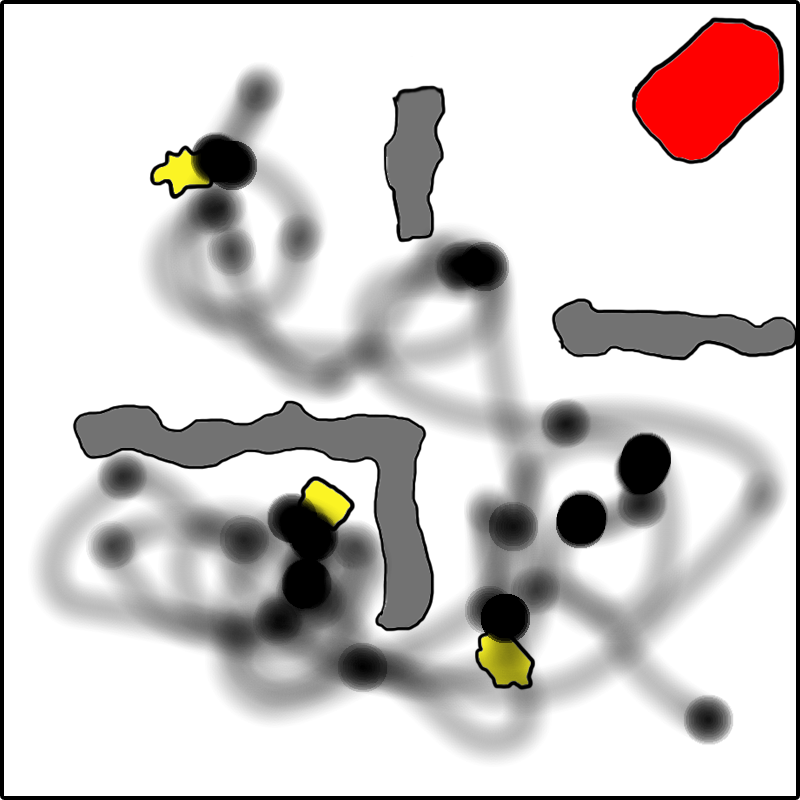
\includegraphics[width=0.4\textwidth]{contents/testing/heatmaps/imachination/8Dai.png}}               \qquad
  \subfloat[Uden KI]{\label{fig:ima8Dnoai}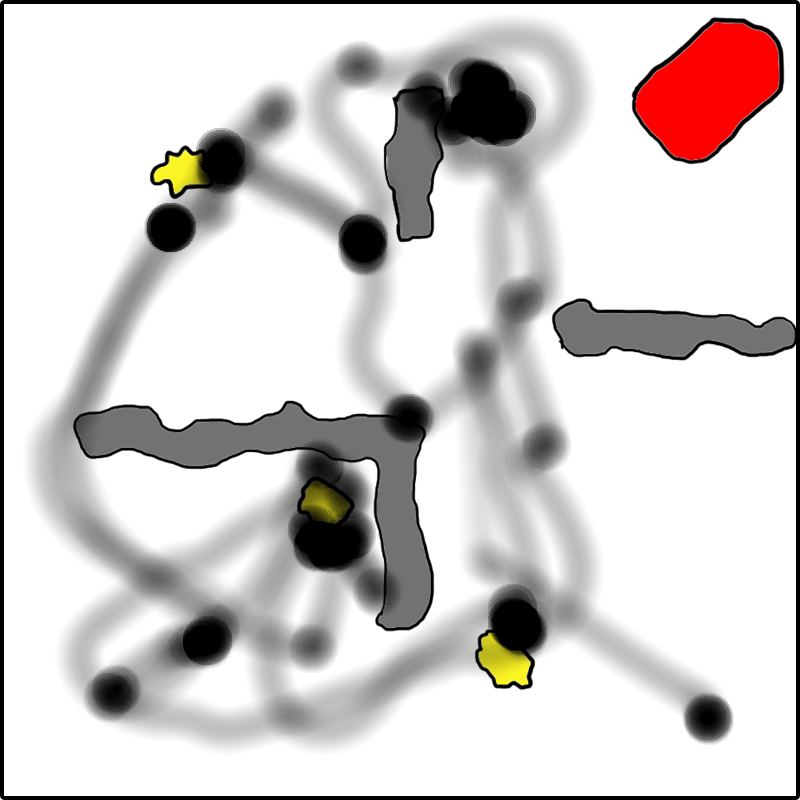
\includegraphics[width=0.4\textwidth]{contents/testing/heatmaps/imachination/8Dnoai.png}}
  \caption{8D spillede uden KI f�rst}
  \label{fig:8Dima}
\end{figure}

\begin{figure}[h]
  \centering
  \subfloat[Med KI]{\label{fig:ima9Dai}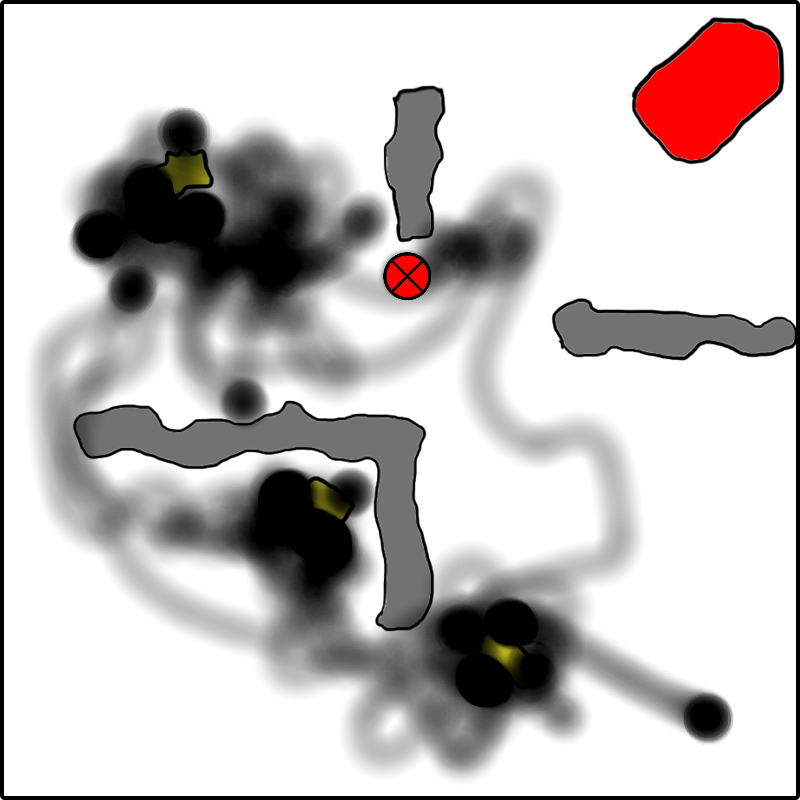
\includegraphics[width=0.4\textwidth]{contents/testing/heatmaps/imachination/9Dai.png}}               \qquad
  \subfloat[Uden KI]{\label{fig:ima9Dnoai}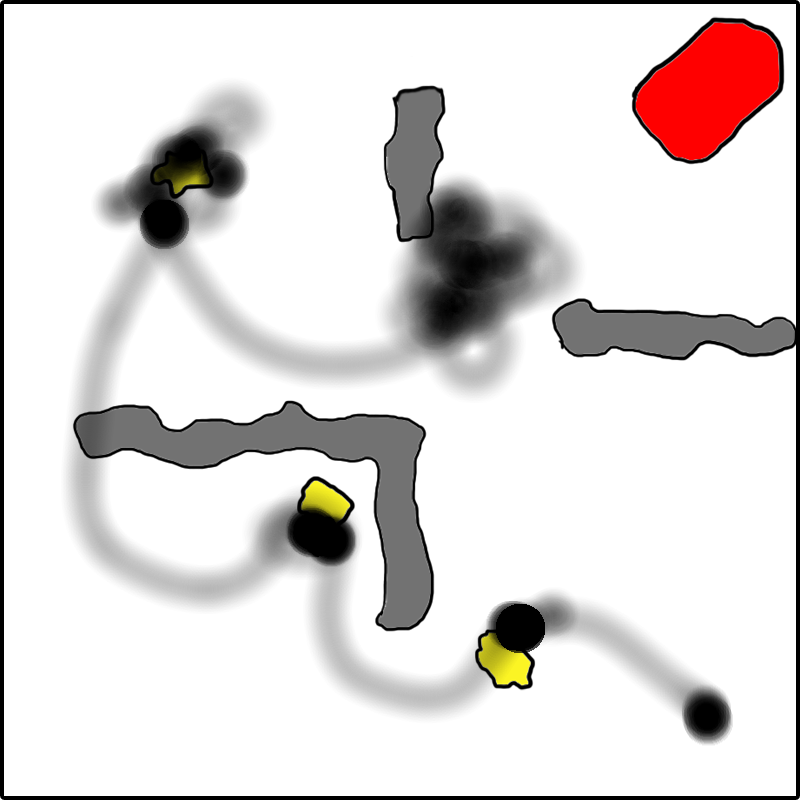
\includegraphics[width=0.4\textwidth]{contents/testing/heatmaps/imachination/9Dnoai.png}}
  \caption{9D spillede uden KI f�rst}
  \label{fig:9Dima}
\end{figure}

\section{\sop}

\section{\cat}

%%% Local Variables: 
%%% mode: latex
%%% TeX-master: "../../report"
%%% End: 
